\chapter{Research}

\section{Previous work}
Some experimentation was already done by BTG before the start of the project that attempted to automate the manual process of configuring a camera.
This only goes as far as writing a script for a specific situation that makes an API call for a specific setting so multiple cameras of the same type can be changed in one go.
While this makes it a little less time consuming to change a setting across all cameras this does not solve the problem of the lack of an overview of the current configuration nor is it user-friendly requiring an engineer to write a script each time a setting needs to be changed.

\section{Focus group}
To better define what the project deliverables would be, a focus group was formed consisting of the graduate student and  Wouter Horlings and Silke Hofstra, who are software engineers at BTG.
During the group sessions it was determined that a system should be implemented capable of configuring a camera in such a way that the configuration does not explicitly need to specify what model of camera is being configured.
The assumption can be made for this project that both cameras are similar in operation but different in configuration but it would be nice if the system could be easily extended to support devices with different capabilities.
This could be done by separating the configuration parameters into generic options and letting the camera specific configuration code determine what options are needed for that particular camera to configure it according to those options.
The focus group also determined that it is desired to be able to rollback a camera configuration using some sort of version control system in case a change to the configuration presented problems.

% Indicated that:
% Takes a lot of work to manage cameras
% The ability/flexibility to configure cameras is not sufficient
% Improvements can be made
% Its difficult to maintain an overview of what templates are being used
% There is not version control
% Current tooling can not work with batches
% Rec: Look at Hikvision Batch Configuration

% What parameters could be relevant?
% Autofocus/zoom
% Video settings (e.g. Bitrate)
% Netwerk settings (suggested, but out of scope)
% Detection sensitivity, to limit alarms sent to the dispatches
% Would be nice to have the ability to quickly change these (overnight) to balance alarm frequency and flase alarms

% Concern about mapping settings between cameras
% Idea with Wouter was to allow this to be configured inside the API.+ Not part of interview though.
% Example map mismatch: Field of view differences between VCA and Hikvision
% TODO Design phase not clear
\section{Interview}
To gain a better insight of the camera configuration related problems experienced by the product organization an interview was conducted with Alex van der Leij, a product manager responsible for the video masts deployed around Europe.
During the interview he indicated that it currently takes a lot of work to manage
the cameras and that the current method of configuring cameras is not flexible enough which could be improved upon. He explained that the way the cameras are currently being
administered is to configure a camera with a set of default settings which are to be considered a set of 'base settings'. These can then be exported to a file which is used as a
'template' for other
cameras. A downside of this approach is that it is difficult to maintain different versions of these files and that it can't easily be determined what version a camera is using.
Another problem he indicated was that current tooling does not provide a practical way to make a single change to a batch of cameras.


After introducing the goal of the project the question was asked as to what parameters he would find valuable to have in the initial prototype.
The parameters that were named as candidates were: automatic camera focus and zoom, video quality, network configuration and detection sensitivity.
Out of these parameters some of them were of particular interest to him. The first one being video quality. It would be nice to configure video quality related settings like a
cameras bitrate and resolution because video masts may be in locations with reduced cellular network connectivity. In that case it would be beneficial to lower the video quality
for these cameras to reduce network load. The second parameter of interest was detection sensitivity. This parameter regulates how sensitive a camera is to movement before it
triggers an alarm to the dispatchers to attract their attention. It would be nice to quickly change this parameter so that the frequency of alarms and false alarms can be balanced.


At the end of the interview some concerns were raised by Alex about how settings might be implemented differently by camera manufacturers. For example a sensitivity setting of 10
on camera A might not cause the same behavior if the same value is used for camera B. A solution to this problem should be found and is described in chapter \ref{sec:design}.

%\section{How should a configuration be represented to express settings for different cameras?}
%The camera configurations should be represented in a generic way so that they can be applied to different cameras. There also needs to be a way to detect if a camera
%has gone out of sync with the stored configuration and a way to revert configurations to previous revisions in case an erroneous setting was applied. To make this comparison the assumption is made that settings can be read back from the cameras using their APIs.

\section{Available product analysis}
Before the design and implementation of the prototype were made, an analysis on already available products was done to see if there were any existing solutions that could be used to satisfy the objective or provide a partial solution to the problem.

As part of the analysis an online search was conducted using search terms like "camera lifecycle management software", "camera configuration tool" and "universal ip camera configuration tool".
This search led to results of some tools that could discover IP cameras using protocols like Bonjour, ONVIF Device Discovery or UPnP but none of these tools provided a capability to configure a camera as can be done with the built-in browser based interface of the camera or the manufacturer provided API.
Because no existing solution satisfied the needs of the stakeholders the search was broadened to other kinds of lifecycle management software to see if some of the concepts could be applied to a new system aimed at configuring cameras. 
A solution was found that implemented a templating system aimed at configuring Unix-like and Windows servers.
This solution is called Foreman.

,,Foreman is an open source project that helps system administrators manage servers throughout their lifecycle, from provisioning and configuration to orchestration and monitoring." \cite{noauthor_foreman_nodate}
The project gives the administrator the ability to automate repetitive tasks by supporting an interface with common configuration management solutions like Puppet, Ansible, Chef and Salt.

In addition to being a frontend to these configuration management solutions Foreman also provides a host management system known as ,,Host Groups" \cite{noauthor_foreman_nodate-1}. In this context a host is any Linux client that Foreman manages.
A host group functions as a template for common host settings.
Hosts that have been assigned to a host group inherit any settings that have been defined in that group.
Host groups can also be nested into a hierarchy.
This way the topmost host group can serve as a base level group containing general settings for all hosts.
The host groups that have been nested under this group will inherit its settings but also allow the administrator to provide more specific settings for that group.
For example one could have a base level host group that defines the settings for the operating system, and nested host groups can define settings for the software running on that system.

While Foreman uses these host groups for defining parameters for operating systems this concept also translates to other types of systems.
Because of that the choice is made to use these host groups as the basis for designing the templating system for the cameras.

\section{Revision history}
As was indicated by the focus group there should be a way to keep a revision history between templates.
When a change to a template turns out to be problematic it should be possible to revert it to an earlier revision.
Furthermore it should also be possible to know who made a change and with what intention.
To determine the best way to implement this a couple of option were evaluated.

\subsection{One file per revision}
The first option that was evaluated was to use one file per template revision.
Using this method templates would be stored in a directory named after the template.
Inside that directory a template is stored as a file named with the revision number and the file extension.
This way the latest revision can be found by sorting the files by name in descending order.
When a template is reverted to a previous version the files could be sorted in the same manner and will be deleted or otherwise marked inactive until the revision to be reverted to is reached. An example of how this directory structure would be stored is seen in figure \ref{fig:diskstruct}

\begin{figure}[h!]
	\centering
	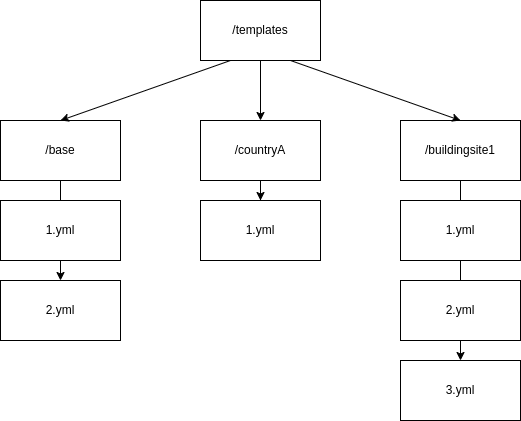
\includegraphics[scale=0.5]{yaml_dir_struct}
	\caption{Directory structure of templates and their revisions using one file per revision.}
	\label{fig:diskstruct}
\end{figure}

Storing templates in this manner has one flaw.
Namely that of sorting by name when more than 10 revisions have been made.
When sorting the files by name the tenth revision would be sorted between files starting with 1 and 2.
In this case the descending sorted order would then be: 9, 8, 7, 6, 5, 4, 3, 2, 10, 1.
This could be prevented by adding leading zeroes to the filename but that only delays the problem until the amount of revisions overflows the leading zeroes.
If for example four digits would be used where the unused digits are zeroed the descending sorted order would be: 0010, 0009, 0008, 0007, 0006, 0005, 0004, 0003, 0002, 0001.
As can be seen this would solve the problem but as soon as more than 9999 revisions are made the same problem occurse.
Another potential solution unaffected by this problem is the use of the file modification time as stored on the filesystem.
Using this file attribute would work in most cases although it can be affected by external factors such as changing system time or restoring from backups where the proper file attributes are not restored \cite{noauthor_mtime_nodate}.

\subsection{Git}
The second option that was evaluated was to use git.
While git is most often used for tracking changes in software source files it describes itself as a fast, scaleable, distributed revision control system or "stupid" content tracker, since it makes no assumption about what content is stored in it \cite{truyers_git_2016}.

Git can be used to keep track of changes in a repository by chaining them into commits.
Each commit contains a snapshot of a set of files, a message that gives a description about the changes and metadata like who made a change and when.
When a new commit is made a reference to that commit is stored that tells you what the latest commit in the chain is.
This reference is called the HEAD and can be seen in figure \ref{fig:gitcommit}.
By changing what commit the HEAD points to you can revert the state of the files in your repository back to an earlier commit.

\begin{marginfigure}
	\centering
	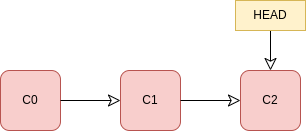
\includegraphics{git_commit}
	\caption{The HEAD is moved to the latest commit.}
	\label{fig:gitcommit}
\end{marginfigure}

Normally a user of git would interact with the repository through a command line or graphical user interface using a set of commands.
There are many different commands that are available to the user.
Examples of the most commonly used commands to view and record changes are: `git add` to mark files to be comitted (called staging), `git commit` to commit all the files that have been staged, `git push` to upload local changes to a remote git repository and `git status` to get a brief summary of that state of the repository. There are many more commands that can be used but for the purposes of brevity these have been omitted.

Several libraries exist that implement these commands and allow us to use git from a program to make commits of our data and to revert back to an earlier version if necessary.
Some notable ones are libgit2\footnote{\url{https://github.com/libgit2/libgit2}}, a pure C based implementation, and go-git\footnote{\url{https://pkg.go.dev/github.com/go-git/go-git/v5}}, an implementation in the Go programming language.

Git makes a distinction between two types of commands.
The first type of command categorizes the most commonly used high-level commands which have been described earlier and are called "porcelain" functions.
The second type involves the low-level functions that directly modify git's internal datastructure and are called "plumbing" functions.
These plumbing functions are normally used by the "porcelain" functions to implement their behavior but they can also be used for more advanced usecases where the porcelain function are not sufficient.

Storing program data using git's porcelain functions carries the potential for optimization by using git as a "bare" repository using the plumbing functions.
This way all files exist only within the git database instead of the filesystem.
A method of using the plumbing functions to directly create blobs in git's database and essentially turning it into a NoSQL database is described in an article by Kenneth Truyers\cite{truyers_git_2016}.

%How would this work using plumbing functions to optimize \cite{noauthor_git_2016}
%In short: By using a plain git repository there are a couple of disadvantages.
%All data needs to be written to disk before they can be added to git.
%Data is saved multiple times, once as a file and again in git as a blob.
%There is no data deduplication.
%
%Conclusion of this: using plumbing commands provides some optimizations but it requires quite a bit of work to implement.
%Because of that the choice is made to use a simple git repo for the prototype but suggest this optimization as a future improvement in the Recommendations chapter...
%
%all files need to be sorted
%git gives it to you instantly
%difficult to diff
%proven to work
%possibility for backups
%
%
%Argument: Is git overkill? Why use it or the other suggested solution. Make a choice.
%
%
%NoSql object database?
%Maybe also look at more classical databases like sql/Mongodb? - no experience and the requirement state a human readable format which a database is not.
%Does it allow revisions?
%
%Possible optimizations
%
%Revision can be stored in git or as separate files
%With git the choice can be made between using the porcelain functions to add files and commit them or to use the internals to manually create blobs.
%The latter has the advantage of not having an extra working copy but requires more work and may introduce more programming errors.
%
%The way these could be stored on disk are having multiple templates in the same directory, having a separate directory for each template or putting all templates in the same file.

\subsection{Conclusion}
Looking at both of these options it is evident that the manual approach of using numbered files has some undesirable effects.
Because of that the choice is made to implement revisions using git's porcelain functions.
While the approach of using plumbing functions with a bare git repository would also be a suitable solution it would take more time to implement.
Considering that only a prototype will be built that uses just a handful of templates the benefits of using the plumbing functions are considered to be negligible and would not outweigh the time needed to implement it.
